
O setor de jogos digitais está expansão, prevendo-se que ultrapasse os US\$ 200 bilhões em 2023, conforme indicação de \citeonline{quanto_games_vao_movimentar}. No ano de 2022, somente na plataforma Steam, foram lançados 10.644 novos títulos, e em 2023 até seis de Outubro foram lançados 9,103 jogos, conforme evidenciado pela \cref{fig:steam_publishes} existe uma tendência do aumento de lançamentos de jogos na Steam ao decorrer dos anos.


\begin{figure}[!ht]
	\centering
    \caption{número de jogos publicados na Steam.}
	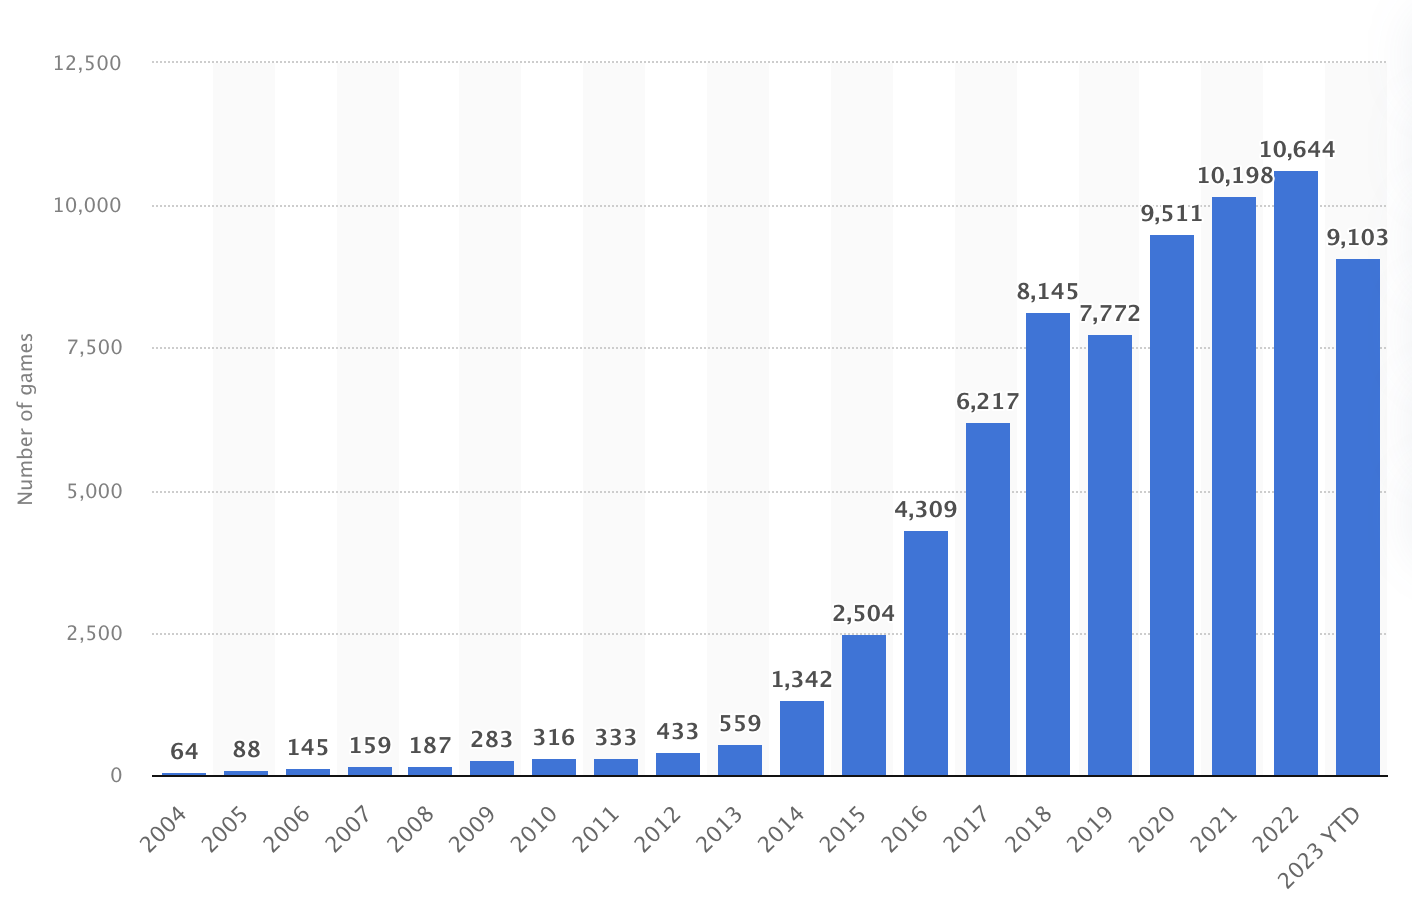
\includegraphics[width=0.6\textwidth]{figures/steam_sales.png}
	\legend{Fonte: \citeonline{numero_de_jogos_publicados_na_steam}}
	\label{fig:steam_publishes}
\end{figure}

Dentro do universo dos jogos, os mapas assumem um papel fundamental, não apenas orientando os jogadores, mas também enriquecendo a experiência ao criar uma sensação de escala e proporcionar uma exploração mais rica \space\cite{video_game_maps, minimap}.

Na elaboração de mapas, emprega-se uma técnica denominada geração procedural, a qual se baseia na criação dinâmica de conteúdo por meio de algoritmos. Essa abordagem surgiu com o propósito de gerar mapas durante a execução de um programa e minimizar as demandas de armazenamento, uma vez que havia restrições nesse aspecto na época. Contudo, mesmo diante da superação dessas limitações nos dias atuais, a geração procedural persiste como uma estratégia aplicada para a produção de conteúdos exclusivos a cada execução do programa \cite{kenny2021procedural}.

% No cenário de jogos, os mapas desempenham um papel fundamental, fornecendo orientação aos jogadores e criando a sensação de escala em uma área. Por exemplo o jogo de aventura pirata chamado Sea of Thieves, os mapas revelam locais de interesse, como tesouros escondidos, missões e áreas perigosas, além de ajudar os jogadores a planejar suas estratégias, explorar o mundo virtual e tomar decisões com base em informações espaciais. Portanto os mapas enriquecem a experiência geral do jogo, mas cria-los pode ser um desafio, especialmente levando em consideração o orçamento disponível. Pois demandaria muitos recursos criar vários mapas diferentes com intuito de entretenimento do jogador. Em jogos como Minecraft, um elemento importante é a geração procedural, que consiste em um conjunto de algoritmos e ferramentas para geração de conteúdo, no qual se cria os mundos, com ilhas contendo biomas, cavernas, vilas, dentre outros recursos. Com essa diversidade de características pode-se evitar o tédio de sempre jogar no mesmo mapa \space\cite{video-game-maps, lecafedugeek}.


"Um dos maiores desafios  no desenvolvimento de algoritmos para geração de mapas é  a  dificuldade  de  se  criar  cenários  que  sejam,  ao mesmo  tempo,  atraentes  e diversificados,  permitindo que o jogador possa explorar um novo ambiente a cada sessão de jogo" \space\cite{geracao_procedural_jogos_2d}.

Contextualizando, a área de Geometria Computacional é um ramo da ciência da computação que estuda algoritmos e estruturas de dados, servindo para resolução computacional de problemas geométricos. O diagrama de Voronoi é um dos tópicos mais discutidos dessa
área e possui uma gama de utilizações, dentre elas pode ser utilizado para resolver alguns problemas relacionados a jogos como por exemplo marcar pontos em um plano, desses pontos criar regiões, e a partir dessas regiões criar biomas gerando um mapa \space\cite{rodrigues_diagrama_2019}.


De acordo com \citeonline{jogo_procedural} é muito comum usar técnicas procedurais combinado com Inteligência Artificial (IA) para melhorar ou personalizar a experiência do jogador. Por exemplo, o jogo RimWorld é um simulador de colônia que gera um planeta de forma procedural e utiliza uma IA para narrar a história, abrangendo psicologia, ecologia, combate e diplomacia, dentre outros. Logo, essa combinação entre IA e a geração procedural cria uma jogabilidade única ao jogador.


Em IA, um ramo que está em ascensão é o de segmentação de imagem com redes neurais convolucionais, que constitui-se em classificar os pixeis de uma imagem ou criar áreas na imagem para destacar cada objeto (todas classes que são contáveis como pessoas, carros, etc) detectado ou até mesmo mesclar essas duas técnicas. Neste ramo existem diversas aplicações, como por exemplo carros autônomos e sistemas de vigilância.
Na aplicação de carros autônomos é necessário identificar humanos para tomar decisões de freio, em sistemas de vigilância é necessário identificar para alertar e automatizar o processo de segurança. Portanto, nessas aplicações reais observa-se a importância em identificar seres humanos para a tomada de decisões \space\cite{dp_semantic_segmantation}.


Com base na contextualização é possível perceber que o mercado de jogos está em ascensão, o mapa é um recurso importante e pode ser usado a técnica de geração procedural para diversificar, o diagrama de Voronoi pode ser usado para gerar biomas em mapas no processo de geração procedural, a técnica de geração procedural de conteúdo unido a inteligência artificial é muito utilizado em jogos para criar personalizações, no ramo de inteligência artificial a segmentação com redes neurais convolucionais está em destaque. Logo pode-se perceber a relevância desses temas no curso de ciência da computação e na atualidade, propõe-se então, uma solução para personalizar mapas de jogos utilizando um modelo de IA da área de segmentação usando redes neurais convolucionais.

Com o objetivo de gerar mapas com biomas de forma procedural com personalização de IA, decidiu-se utilizar o resultado da segmentação de imagem por rede neural convolucional para o usuário selecionar uma área e assim delimitar o contorno da ilha, adicionando, portanto, uma personalização. Essa aplicação possibilita um desenvolvedor de jogos criar um protótipo de mapa rapidamente ou aprimorar e usar esse recurso no jogo, possibilitando o jogador tirar ou selecionar uma foto e escolher um contorno para gerar um mapa com aquele formato.

Por fim, para contribuição científica tem-se a hipótese de que quanto mais pontos o diagrama de Voronoi tiver maior será a precisão da compatibilidade entre o mapa gerado e o contorno escolhido. Para chegar a essa conclusão, comprometeu-se definir alguns testes com métricas em prol de mensurar a qualidade da geração procedural com o contorno selecionado.

\section{Objetivos}

O objetivo principal deste trabalho é desenvolver uma ferramenta que ofereça uma alternativa para a geração procedural de mapas de ilhas, utilizando o diagrama de Voronoi para a criar biomas. Além disso, pretende-se combinar segmentação com redes neurais convolucionais para permitir a personalização desses mapas. Essa ferramenta terá a capacidade de reconhecer os contornos reconhecidos (classificados no conjunto de dados, logo o resultado terá uma detecção abrangente dentro do escopo de classes obtidas) de uma imagem, e gerar um mapa com um mapa baseado nos limites do contorno escolhido.

Adicionalmente, os seguintes objetivos específicos serão abordados:

\begin{itemize}
	\item Selecionar e analisar conjuntos de dados contendo classes relevantes, como pessoas, carros, entre outros, para treinar um modelo de rede neural convolucional específico para segmentação de imagens.
	\item Utilizar algoritmos para criar diagramas de Voronoi.
	\item Aplicar um algoritmo para reconhecer a imagem com o contorno selecionado e gerar como resultado a imagem do mapa gerado.
	\item Utilizar o resultado da segmentação para selecionar indicar o que é terreno em cima do diagrama de Voronoi.
	\item Gerar os biomas no diagrama de Voronoi.
	\item Criar testes em prol de mensurar a semelhança entre o contorno do mapa gerado com o contorno escolhido.
\end{itemize}